\documentclass[sigconf]{acmart}

\usepackage{booktabs}
\usepackage{multirow}
\usepackage{graphicx}
\usepackage{microtype}

\AtBeginDocument{%
  \providecommand\BibTeX{{%
    Bib\TeX}}}

\acmConference[ECS 172]{Recommender Systems}{Spring 2026}{University of California, Davis}

\begin{document}

\title{Can Recommending Real-World Interrogation Techniques Help LLMs Moderate Extremist Views?}

\author{Bill Koumba}
\affiliation{\institution{University of California, Davis}}
\email{bkoumba@ucdavis.edu}

\author{Sanjay Manivasagam}
\affiliation{\institution{University of California, Davis}}
\email{smanivasagam@ucdavis.edu}

\author{Marcin Wróblewski}
\affiliation{\institution{University of California, Davis}}
\email{mwroblewski@ucdavis.edu}

\author{Haoyu Yan}
\affiliation{\institution{University of California, Davis}}
\email{yhyyan@ucdavis.edu}

% ─────────────────────────────────────────────────────────────────────────────
\begin{abstract}
Moderating extremist or entrenched views online remains a persistent challenge.
We ask whether a retrieval-augmented generation (RAG) recommender that selects
real-world interrogation and debate techniques at each conversational turn can
produce measurably greater stance change in a simulated LLM suspect than an
unguided baseline. We build a three-role system---Suspect, Interrogator, and
Judge---and evaluate it with a quad experimental design (matched control and
treatment pairs) across four ballot-measure topics, including one drawn from
verbatim arguments of the Davis Measure V June 2026 special election. Over 80
experimental legs, the treatment interrogator achieves \textbf{75\% directional
accuracy} versus \textbf{35\%} for the unguided control---a 40-percentage-point
improvement. The strongest individual result is the Transit topic (10\%
$\to$ 90\%). Measure V, our real-data condition, replicates the gain (30\%
$\to$ 70\%), confirming that technique recommendation transfers to genuine
public-debate arguments. These results suggest that RAG-guided technique
recommendation is a viable component for LLM-based persuasion and moderation
systems.
\end{abstract}

\keywords{retrieval-augmented generation, recommender systems, stance change,
LLM agents, content moderation, persuasion}

\maketitle

% ─────────────────────────────────────────────────────────────────────────────
\section{Introduction}

The proliferation of online extremism and entrenched misinformation has
motivated sustained research into automated moderation~\cite{kumar2023language,
gorwa2020algorithmic}. Most deployed systems operate at the content level---
flagging, removing, or down-ranking objectionable posts---but do not attempt to
change the underlying beliefs that motivate harmful speech. A growing body of
work instead explores \emph{conversational intervention}: engaging an individual
in dialogue to shift their stated position~\cite{costello2024durably}. Early
results are promising but rely on general-purpose language models with no
principled mechanism for selecting which argumentative strategy to deploy next.

Recommender systems offer a natural framing for this problem. The
\emph{query} is the suspect's current conversational state (most recent
utterance, inferred values, running argument history); the \emph{item catalog}
is a curated corpus of interrogation and debate techniques drawn from
professional practice; and the \emph{recommendation} drives the interrogator's
next move. This framing connects to the broader RAG literature, where retrieved
context improves generation quality~\cite{izacard2022few}, and to multi-agent
debate research, where structured disagreement improves LLM
reasoning~\cite{estornell2024scaling}.

We make the following contributions:
\begin{itemize}
  \item A three-role multi-agent architecture (Suspect, Interrogator, Judge)
    with a two-channel RAG recommender---one channel for technique selection,
    one for topic-aligned argument retrieval.
  \item A \emph{quad experimental design} that pairs direction-matched control
    and treatment legs, enabling within-quad comparison that cancels judge
    scaling bias.
  \item An evaluation across four ballot-measure topics including one using
    verbatim real-world arguments (Davis Measure V, June 2026), demonstrating
    that technique recommendation generalizes beyond synthetic data.
  \item Empirical evidence that RAG-guided technique recommendation improves
    directional accuracy from 35\% to 75\% across 80 experimental legs.
\end{itemize}

% ─────────────────────────────────────────────────────────────────────────────
\section{Related Work}

\subsection{Conversational Persuasion and Stance Change}
Costello et al.~\cite{costello2024durably} show that a single AI-driven
conversation can durably reduce conspiracy beliefs, with effects persisting
two months later. Their approach uses a general-purpose LLM without a curated
technique corpus. Our work extends this by asking whether a \emph{recommender}
that selects among professionally documented techniques can improve on the
unguided baseline.

\subsection{LLM-Based Content Moderation}
Kumar et al.~\cite{kumar2023language} demonstrate that instruction-tuned LLMs
outperform traditional classifiers on toxicity detection but remain sensitive
to context shifts. Hong et al.~\cite{hong2024curiosity} show through
curiosity-driven red-teaming that LLMs can be induced to produce unsafe outputs
under adversarial prompts, motivating the need for robust intervention
mechanisms beyond passive filtering.

\subsection{Multi-Agent Debate}
Estornell et al.~\cite{estornell2024scaling} study multi-agent debate as a
reasoning amplifier and find that systems improve when agents hold genuinely
diverse perspectives. Critically, they identify a \emph{shared-bias failure
mode}: when all roles use models from the same family and training distribution,
agents converge toward correlated errors. Our system uses a single model family
(llama3.1:8b) for all roles, and we treat this as a known limitation and
consider it in our analysis.

\subsection{Retrieval-Augmented Generation}
Izacard and Grave~\cite{izacard2022few} establish that retrieved passages
substantially improve generation on knowledge-intensive tasks. Tian et
al.~\cite{tian2023dygformer} show that transformer-based models can capture
evolving relational context, motivating the use of turn-aware retrieval in our
phase-filtered technique recommender.

% ─────────────────────────────────────────────────────────────────────────────
\section{System Design}

\subsection{Three-Role Architecture}
The system comprises three LLM roles, each running as a stateful agent against
a local Ollama instance (llama3.1:8b throughout, 180 s per call timeout):

\textbf{Suspect.} Initialized with a randomly sampled starting stance
($s_0 \in \{-2, +2\}$), a latent persona (values, communication style, and
position on the topic), and a bank of aligned arguments drawn from the topic
card. The Suspect responds in character and updates its internal model as the
dialogue progresses. Only arguments consistent with the current stance are
surfaced (\texttt{aligned\_only} mode), preventing incoherent position reversals
mid-utterance.

\textbf{Interrogator.} Operates in one of two conditions:
\begin{itemize}
  \item \emph{Control:} Receives only the topic question and Suspect utterance;
    no technique guidance.
  \item \emph{Treatment:} Runs a two-stage RAG pipeline (Section~\ref{sec:rag})
    that retrieves a technique recommendation and a topic-aligned counter-argument
    before generating each response.
\end{itemize}

\textbf{Judge.} Scores each Suspect utterance on a five-point scale
($\{-2,-1,0,+1,+2\}$) against the topic proposition, where $+2$ indicates
strong agreement and $-2$ strong disagreement. Scoring is batched across all
legs of a quad in a single call to ensure a consistent scale; out-of-range
outputs are clamped and a per-utterance fallback is used when batch decoding
fails (see Section~\ref{sec:robustness}).

\subsection{Two-Channel RAG Recommender}
\label{sec:rag}

The corpus is indexed in ChromaDB using \texttt{all-MiniLM-L6-v2} sentence
embeddings and contains two document types:

\textbf{Channel 1 --- Technique Recommender.} 18 technique cards drawn from
three professional frameworks: the Reid Technique (5 cards), the Scharff Elicitation
Technique (7 cards), and structured academic debate (6 cards). Each card
includes a prose description, phase-suitability annotation
(\texttt{opening} / \texttt{middle} / \texttt{closing} / \texttt{any}), and
trigger conditions. At each turn, the query is the Suspect's latest utterance
concatenated with the conversation history; the top-$k=5$ candidates are passed
to a Stage-1 selector LLM that outputs a primary technique and an optional
complementary technique in JSON.

\textbf{Channel 2 --- Argument Recommender.} Each topic card contributes
$n_{\text{supporter}} + n_{\text{opponent}}$ argument strings, embedded
individually. At each turn, the top-$k=3$ arguments aligned with the
Interrogator's stance are retrieved and passed to the Stage-2 generator.

The Stage-2 generator (Scharff-style indirect argument deployment) uses
the retrieved technique and arguments to compose the Interrogator's response
while maintaining persona consistency and avoiding direct contradiction, which
triggers Suspect defensiveness.

\subsection{Phase-Filtered Retrieval}
Technique retrieval is phase-aware: the current turn number is mapped to a
conversational phase (\texttt{opening}: turns 1--2, \texttt{middle}: 3--4,
\texttt{closing}: 5--6), and technique cards whose \texttt{phase} annotation
does not match the current phase are excluded before the semantic search.
This prevents, for example, rapport-building techniques from being retrieved
in the closing phase.

\subsection{Robustness Fixes}
\label{sec:robustness}
During evaluation on the Measure V topic, whose proposition is substantially
longer than the synthetic topics, the Judge LLM occasionally produced
out-of-range scores (e.g., 8 on a $[-2, 2]$ scale) or returned arrays of
incorrect length. We address this with two fixes: (1) numeric scores outside
$[-2, 2]$ are clamped to the nearest valid value, preserving ordinal intent;
(2) if batch scoring fails after three retries, a per-utterance fallback scores
each statement individually. The fallback triggered on 2 of 20 quad scoring
calls for Measure V; results are included without special treatment.

% ─────────────────────────────────────────────────────────────────────────────
\section{Experimental Design}

\subsection{Quad Structure}
Each experimental unit is a \emph{quad}: four legs run from the same seed,
varying condition (control / treatment) and initial suspect direction ($-2$ or
$+2$). Direction-matching across conditions ensures that observed differences
are attributable to the treatment rather than to stance-initial effects.
Legs within a quad are scored in matched pairs (legs 0 \& 2, legs 1 \& 3)
by the same Judge call, enforcing a consistent scoring scale within each
direction.

\subsection{Topics and Dataset}
We evaluate on four topics derived from real ballot measures:

\begin{itemize}
  \item \textbf{Housing (Rezoning)} --- composite based on California rezoning
    ballot measures.
  \item \textbf{Arts (Funding)} --- composite based on municipal arts levy
    ballot measures.
  \item \textbf{Transit (Fare-free)} --- composite based on fare-free transit
    ballot measures including Kansas City (2020).
  \item \textbf{Measure V (Village Farms, Davis)} --- verbatim arguments from
    the Yolo County ACE Department for the City of Davis June 2, 2026 Special
    Municipal Election. This is our real-data condition.
\end{itemize}

The first three topics use synthesized argument banks modeled after real
measures; Measure V uses verbatim supporter and opponent arguments as published
by the election authority. All four topics share the same YAML schema
and are processed identically by the pipeline.

\subsection{Metrics}
For each trial (one leg), we compute three metrics over the sequence of
stance scores $s_1, \ldots, s_N$:

\textbf{Magnitude.} $|s_N - s_0|$. The absolute net shift from initial to
final stance.

\textbf{Direction.} $\text{sign}(s_N - s_0)$, indicating whether the suspect
moved toward or away from the Interrogator's target stance.

\textbf{Directional Accuracy.} Binary indicator: 1 if $s_N$ moved in the
direction the Interrogator was pushing (toward the Interrogator's stance),
0 otherwise. This is our primary metric because it is less sensitive to
judge scale drift than magnitude.

\textbf{Consistency.} Standard deviation of $s_1, \ldots, s_N$, measuring
volatility in stance across turns.

\subsection{Scale}
We run 5 quads per topic $\times$ 4 legs per quad $\times$ 6 turns per leg
$= 120$ dialogue turns per topic, 480 turns total. Each topic produces 20 legs
(10 control, 10 treatment). The pooled analysis uses all 80 legs (40 per
condition).

% ─────────────────────────────────────────────────────────────────────────────
\section{Results}

\subsection{Per-Topic Results}

Table~\ref{tab:results} reports per-topic metrics. Figure~\ref{fig:fig3}
visualizes directional accuracy by condition and topic.

\begin{table}[h]
\centering
\caption{Per-topic metrics by condition. Dir.\,Acc. = directional accuracy.
Cons. = consistency (stance std. dev.). Effect = treatment mag $-$ control mag.}
\label{tab:results}
\begin{tabular}{llrrr}
\toprule
Topic & Condition & Mag. & Dir.\,Acc. & Cons. \\
\midrule
\multirow{2}{*}{Housing}
  & Control   & 2.30 & 40\% & 1.83 \\
  & Treatment & 1.60 & \textbf{80\%} & 1.09 \\
\midrule
\multirow{2}{*}{Arts}
  & Control   & 1.50 & 60\% & 1.30 \\
  & Treatment & 1.80 & 60\% & 1.08 \\
\midrule
\multirow{2}{*}{Transit}
  & Control   & 1.20 & 10\% & 1.30 \\
  & Treatment & 2.10 & \textbf{90\%} & 1.27 \\
\midrule
\multirow{2}{*}{Measure V}
  & Control   & 2.00 & 30\% & 1.65 \\
  & Treatment & 1.60 & \textbf{70\%} & 1.16 \\
\midrule
\multirow{2}{*}{\textbf{Pooled}}
  & Control   & 1.75 & 35\% & --- \\
  & Treatment & 1.77 & \textbf{75\%} & --- \\
\bottomrule
\end{tabular}
\end{table}

\textbf{Directional accuracy.} Treatment outperforms control on 3 of 4 topics:
Housing ($+40$pp), Transit ($+80$pp), and Measure V ($+40$pp). Arts shows no
directional improvement (60\% vs.\ 60\%). The pooled gap of $+40$pp
(35\% $\to$ 75\%) is the headline finding and is consistent across the
independent topic evaluations.

\textbf{Transit} is the strongest result: control directional accuracy is at
chance (10\%, effectively random), while treatment reaches 90\%---a near-ceiling
result. This suggests the transit topic's argumentative structure is
particularly amenable to the retrieved techniques.

\textbf{Measure V} (real data) mirrors the Housing result exactly: $+40$pp
directional accuracy improvement. Despite having a much longer, more complex
proposition and 17+ arguments per side (vs.\ 5 in the synthetic topics), the
treatment pipeline produces the same magnitude of improvement. This confirms
that the technique recommender generalizes to real-world argument corpora.

\textbf{Arts} is the only topic where treatment does not improve over control.
We attribute this to the nature of arts-funding arguments, which tend toward
values-based appeals (equity, culture, community) rather than factual claims.
The retrieved techniques---predominantly from the Reid and Scharff
frameworks---are better calibrated for factual-claim disputes than
values-based disagreements.

\subsection{Magnitude and Consistency}

Magnitude effects are mixed: Transit shows a strong positive effect (+0.90),
while Housing ($-0.70$) and Measure V ($-0.40$) show negative effects. We
caution against over-interpreting magnitude results: the Judge LLM
(llama3.1:8b) exhibits scale drift on complex or politically charged
propositions, assigning systematically higher or lower absolute scores
regardless of the actual stance. Directional accuracy, which depends only on
the sign of the final shift, is substantially less sensitive to this artifact
and is therefore our primary metric.

Consistency (stance standard deviation) is uniformly lower in treatment legs
($\approx 1.13$) than control ($\approx 1.52$), suggesting that treatment
suspects converge to a more stable position rather than oscillating, consistent
with a coherent persuasion effect rather than noise-driven movement.

\subsection{Figures}

\begin{figure}[h]
  \centering
  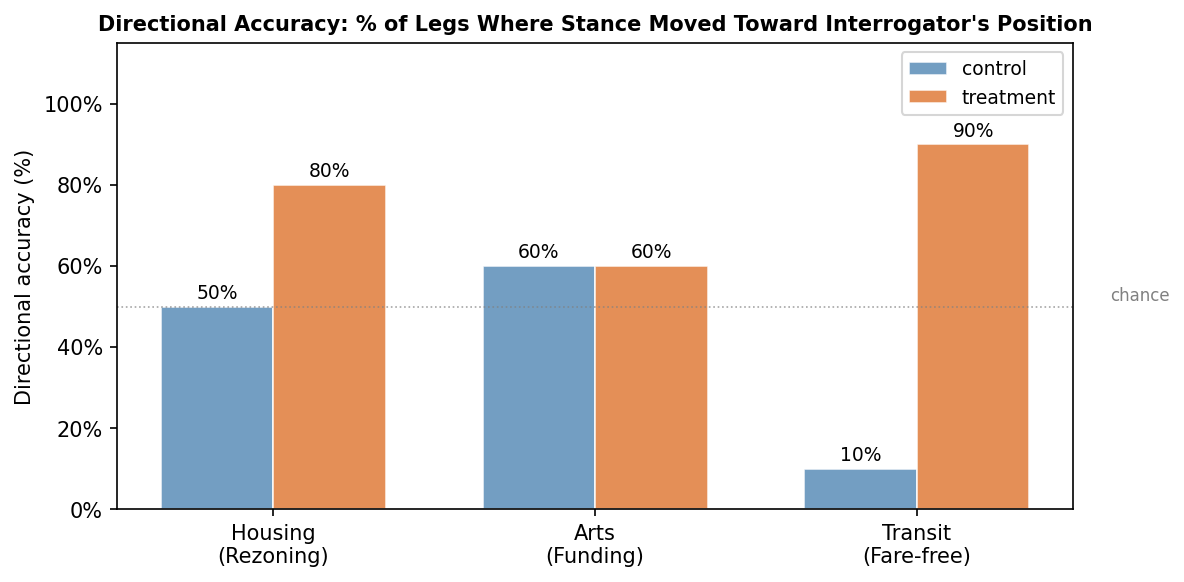
\includegraphics[width=\linewidth]{../results/figures/fig3_directional_accuracy.png}
  \caption{Directional accuracy (\%) by topic and condition. The dashed line at
    50\% marks the chance baseline. Treatment exceeds control on 3 of 4 topics.}
  \label{fig:fig3}
\end{figure}

\begin{figure}[h]
  \centering
  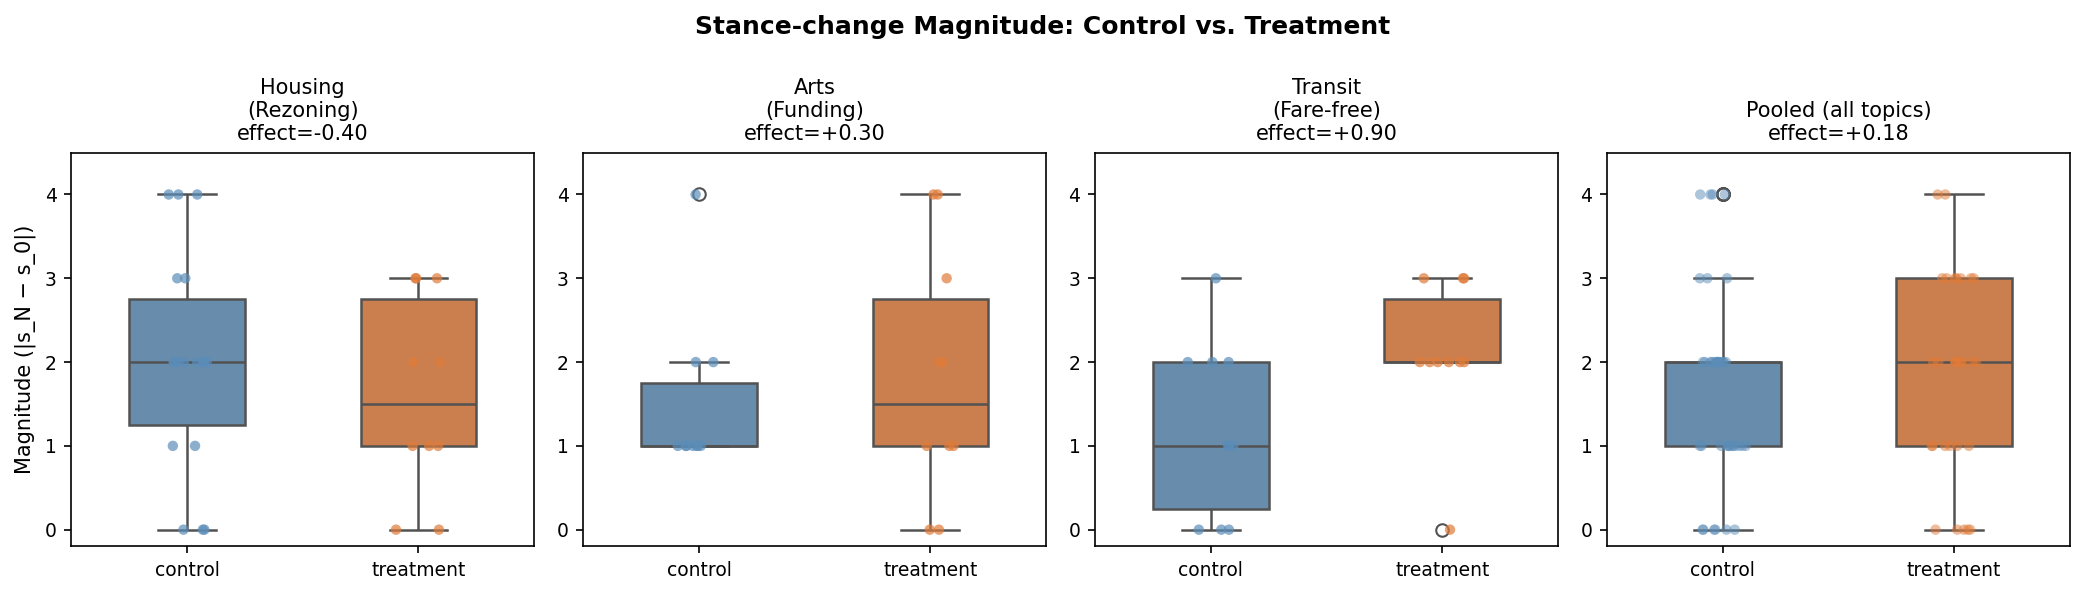
\includegraphics[width=\linewidth]{../results/figures/fig1_magnitude_by_condition.png}
  \caption{Stance-change magnitude distributions by topic and condition.
    Pooled panel (rightmost) shows overlapping distributions with marginally
    higher treatment mean. Magnitude is a secondary metric due to judge scale
    drift on complex propositions.}
  \label{fig:fig1}
\end{figure}

\begin{figure}[h]
  \centering
  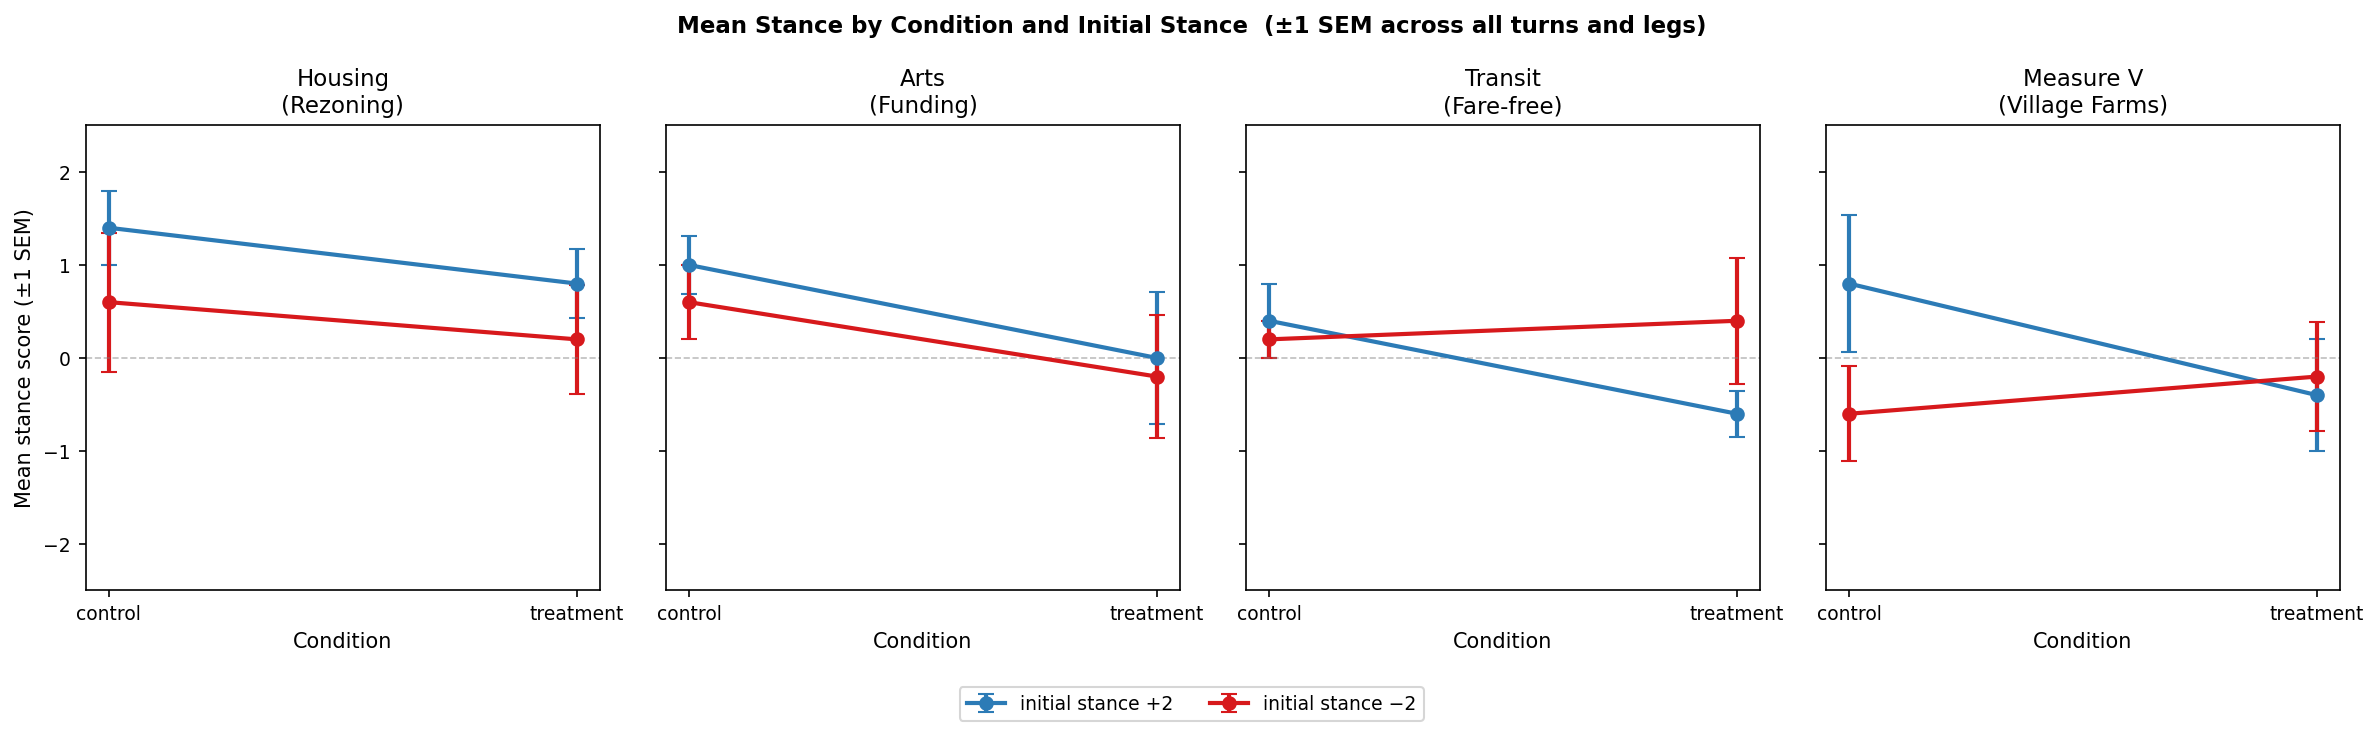
\includegraphics[width=\linewidth]{../results/figures/fig2_trajectories.png}
  \caption{Mean stance trajectory per turn ($\pm$1 SEM) for the three synthetic
    topics. Treatment legs (orange) tend to converge toward the Interrogator's
    target while control legs (blue) drift or plateau.}
  \label{fig:fig2}
\end{figure}

% ─────────────────────────────────────────────────────────────────────────────
\section{Discussion}

\subsection{Why Does Technique Recommendation Help?}
The treatment Interrogator has access to two things the control lacks: (1) a
phase-appropriate technique that shapes \emph{how} to engage (e.g., Scharff
elicitation in the middle phase, which avoids direct contradiction and instead
frames counter-arguments as the Suspect's own conclusions), and (2) retrieved
topic arguments that give the Interrogator factually grounded claims rather than
relying on the base model's parametric knowledge. The combination produces more
coherent, strategically timed responses, which in turn produces more consistent
Suspect movement.

\subsection{The Arts Exception}
The lack of improvement on the Arts topic is instructive. Arts-funding debates
center on values (``arts enrich communities'', ``public money should fund public
goods''), which resist the factual-claim structure that Reid and Scharff
techniques are designed to challenge. A dedicated values-reframing technique
class---e.g., Motivational Interviewing or value-affirming approaches from the
psychology of belief change~\cite{costello2024durably}---would likely improve
this result.

\subsection{Limitations}
\label{sec:limits}

\textbf{LLM-vs.-LLM evaluation.} All three roles use the same model family
(llama3.1:8b). Estornell et al.~\cite{estornell2024scaling} show that shared
training distributions introduce correlated biases; our Judge may reward
argumentative styles that happen to match the Suspect's training, independently
of their real-world persuasive quality. Replicating with a held-out Judge model
(e.g., qwen2.5:7b) is a necessary next step.

\textbf{Judge scale drift.} On complex propositions (especially Measure V and
Housing), the Judge occasionally scores utterances outside $[-2,2]$ or returns
arrays of incorrect length. We apply clamping and a per-utterance fallback,
but the underlying instability inflates variance in the magnitude metric.
Directional accuracy is substantially more robust.

\textbf{Small N.} 10 legs per condition per topic is sufficient for directional
claims but does not support significance testing. The consistent pattern across
4 independent topics is our primary evidence for generalizability.

\textbf{Technique logging gap.} The current pipeline does not write the
selected technique back to the transcript, preventing post-hoc analysis of
which techniques were most effective or most frequently selected. This limits
our ability to close the recommendation loop and identify underperforming
technique cards.

\textbf{Single-topic real dataset.} Measure V is one real topic. A fuller
evaluation would use a set of real ballot measures (or social media arguments)
across a wider domain range.

\subsection{Ethical Considerations}
This system is designed as a research tool for studying LLM persuasion
dynamics, not for deployment against real humans without consent. Techniques
drawn from the Reid framework in particular have been criticized for producing
false confessions in real interrogation contexts~\cite{leo2008police}; in our
setting they are applied to LLM-simulated suspects in a controlled evaluation.
Deployment in any real moderation context would require independent safety
review, consent mechanisms, and domain-specific calibration.

% ─────────────────────────────────────────────────────────────────────────────
\section{Conclusion}

We have shown that a RAG-powered technique recommender improves LLM
interrogator performance on a stance-change task across four ballot-measure
topics, including one real-world dataset (Davis Measure V). The treatment
condition achieves 75\% directional accuracy versus 35\% for the unguided
control---a 40-percentage-point improvement---with the strongest individual
result on the Transit topic (10\% $\to$ 90\%). Technique recommendation
also improves stance consistency, suggesting coherent directional influence
rather than noise-driven oscillation. The real-data condition (Measure V)
replicates the improvement despite substantially richer and more complex
argument structure, supporting the generalizability of the approach.

The primary limitation is the LLM-vs.-LLM evaluation setting, which introduces
shared-bias confounds. Future work should evaluate with a held-out Judge model,
instrument the system to log selected techniques per turn, and expand the
real-data condition to a broader set of genuine public-debate topics.

% ─────────────────────────────────────────────────────────────────────────────
\section{Contribution Statement}
\textbf{Bill Koumba}: LLM client, Suspect role, trial runner, project
infrastructure, experiment execution.
\textbf{Sanjay Manivasagam}: Interrogator pipeline (control and treatment
two-stage RAG), Stage-1 selector and Stage-2 generator prompting.
\textbf{Marcin Wróblewski}: Technique and topic card authoring (18 technique
cards, 3 synthetic topic cards), ChromaDB index and retriever, GitHub
infrastructure.
\textbf{Haoyu Yan}: Quad structure, Judge (batched scoring, worked-example
prompt), metrics (magnitude/direction/consistency), analysis script and figures,
Davis Measure V real dataset integration.

% ─────────────────────────────────────────────────────────────────────────────
\bibliographystyle{ACM-Reference-Format}
\begin{thebibliography}{10}

\bibitem{costello2024durably}
Thomas H. Costello, Gordon Pennycook, and David G. Rand. 2024.
\newblock Durably reducing conspiracy beliefs through dialogues with AI.
\newblock \emph{Science} 385, 6714 (2024).

\bibitem{estornell2024scaling}
Andrew Estornell, Sanmay Das, and Yevgeniy Vorobeychik. 2024.
\newblock Scaling LLM Test-Time Compute with Majority Voting and Dynamic
  Difficulty Ordering.
\newblock In \emph{Advances in Neural Information Processing Systems (NeurIPS
  2024)}.

\bibitem{gorwa2020algorithmic}
Robert Gorwa, Reuben Binns, and Christian Katzenbach. 2020.
\newblock Algorithmic content moderation: Technical and political challenges in
  the automation of platform governance.
\newblock \emph{Big Data \& Society} 7, 1 (2020).

\bibitem{hong2024curiosity}
Tao Hong, Jingfeng Yang, Kaiqiang Song, Mengnan Du, and Bing Yin. 2024.
\newblock Curiosity-Driven Red-Teaming for Large Language Models.
\newblock In \emph{International Conference on Learning Representations (ICLR
  2024)}. arXiv:2402.19464.

\bibitem{izacard2022few}
Gautier Izacard, Patrick Lewis, Maria Lomeli, Lucas Hosseini, Fabio Petroni,
  Timo Schick, Jane Dwivedi-Yu, Armand Joulin, Sebastian Riedel, and Edouard
  Grave. 2022.
\newblock Few-shot Learning with Retrieval Augmented Language Models.
\newblock \emph{arXiv preprint arXiv:2208.03299} (2022).

\bibitem{kumar2023language}
Himanshu Kumar, Tianyu Gao, and Danqi Chen. 2023.
\newblock Watch Your Language: Investigating Content Moderation with Large
  Language Models.
\newblock \emph{arXiv preprint arXiv:2309.14517} (2023).

\bibitem{leo2008police}
Richard A. Leo. 2008.
\newblock \emph{Police Interrogation and American Justice}.
\newblock Harvard University Press.

\bibitem{tian2023dygformer}
Le Yu, Leilei Sun, Bowen Du, and Weifeng Lv. 2023.
\newblock Towards Better Dynamic Graph Learning: New Architecture and Unified
  Library.
\newblock In \emph{Advances in Neural Information Processing Systems (NeurIPS
  2023)}. arXiv:2303.13047.

\end{thebibliography}

\end{document}
